\documentclass[fontsize=12pt,a4paper]{article}
\usepackage{amsmath}
\usepackage{graphicx}
\usepackage{geometry}
\usepackage{floatrow}
\usepackage{layout}
\usepackage{amssymb} 
\usepackage{multirow}
\usepackage{caption}
\geometry{margin=1in}
\usepackage{authblk}
\usepackage{indentfirst}
\usepackage[singlespacing]{setspace}
%\usepackage[onehalfspacing]{setspace}
\usepackage{array,ragged2e}
\newcolumntype{C}[1]{>{\Centering}p{#1}}
\setlength{\parindent}{0pt}%no indent at the start of a new paragraph
\usepackage[section]{placeins}%restrict floats to subsection, enable \FloatBarrier 
\usepackage{commath}%for \norm{}
\usepackage[
backend=biber,
style=numeric,
sorting=debug
]{biblatex}
\graphicspath{{images/}}
\addbibresource{literature.bib}
\documentclass{article}
\usepackage{scalerel,amssymb}
\def\mcirc{\mathbin{\scalerel*{\circ}{j}}}
\def\msquare{\mathord{\scalerel*{\Box}{gX}}}

\title{Study of the Volume of the John-Löwner Ellipsoid}
\author{Xin Qiu }
\date{May 2020}

\begin{document}

\maketitle

\section{Introduction}

In this study we will invest in Grigory Ivanov's paper "On the Volume of the John-Löwner Ellipsoid".

We will find that the optimal upper bound on the volume of the John ellipsoid of a k-dimensional section of n-dimensional cube is $(\frac{n}{k})^{k/2}$ of the volume of the unit ball in $ \mathbb{R}^n$, and an optimal lower bound on the volumn of the Löwner ellipsoid of a projection of the n-dimensional cross-polytope onto k-dimensional subspace $(\frac{k}{n})^{k/2}$ of the volume of the unit ball in $ \mathbb{R}^n$.

\subsection{Definitions and Notations}
We will prove the volume of the minimal ellipsoid with the center at the origin that covers a set of n vectors in $\mathbb{R}^k$ has a tight upper bound. Here are some definitions and notations we need to know before we start to prove the main theorem:\\

\textbf{John Ellipsoid}: the John Ellipsoid of a convex body K is the ellipsoid of maximal volume contained in K.\\

\textbf{Löwner Ellipsoid}: the Löwner ellipsoid of a convex body K is the ellipsoid of minimal volume containing K.\\

Example:
\begin{figure}[!htb]
\centering
  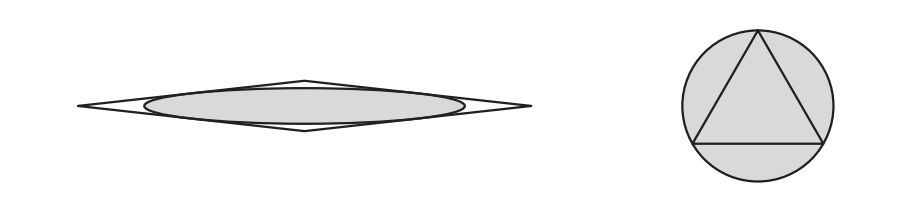
\includegraphics[width=10cm,height = 4 cm]{J-L.PNG}
  \caption{Maximal inscribed ellipse of a flat diamond, and minimal circumscribed ellipse (circle) of a regular triangle}
\end{figure}



\textbf{$H_k$} : k-dimensional subspace of $\mathbb{R}^n$.\\

\textbf{$\varepsilon_{H_k}$}: Löwner ellipsoid of a projection of $\diamond{}^n$ onto $H_k$.\\

\textbf{$\varepsilon^{H_k}$}: John ellipsoid of the section of $\msquare{}^n$ by $H_k$.\\

\textbf{Convex Hull}: A convex hull of a set S in n-dimention is the intersection of all convex sets containing S.\\

\begin{figure}[!htb]
\centering
  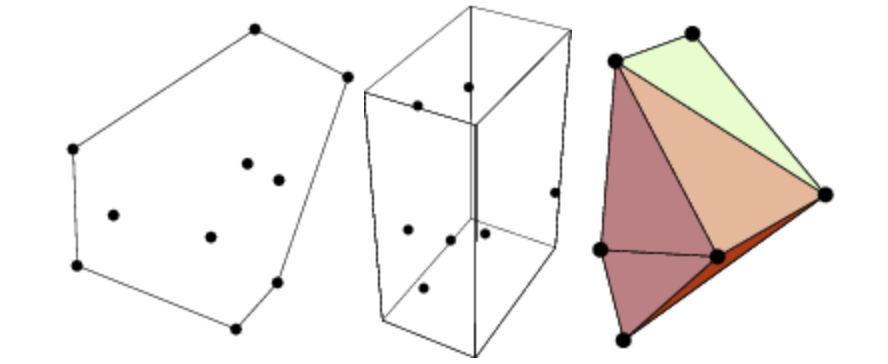
\includegraphics[width=7cm,]{convex-h.png}
  \caption{convex hull examples}
\end{figure}


\textbf{Hypercube}: In geometry, a hypercube is an n-dimensional analogue of a square and a cube. It is a closed, compact, convex figure whose 1-skeleton consists of groups of opposite parallel line segments aligned in each of the space's dimensions, perpendicular to each other and of the same length.\\

\begin{figure}[!htb]
\centering
  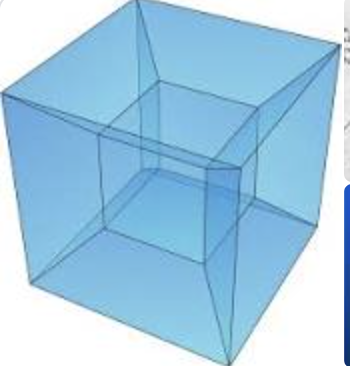
\includegraphics[width=3cm,height = 3cm]{hypercube.png}
  \caption{Hypercube example}
\end{figure}



\textbf{Cross-Polytope} : ($\diamond{}^n$) is a regular convex polytope that exists in n-dimensions. The cross-polytope is the convex hull of its vertices. The n-dimensional corss-polytope can also be difined as the closed unit ball in the $l_1$-norm on $\mathbb{R}^n$:\\
$\{x \in \mathbb{R}^n : \norm{x}_1 \leq 1\}$\\

\begin{figure}[!htb]
\centering
  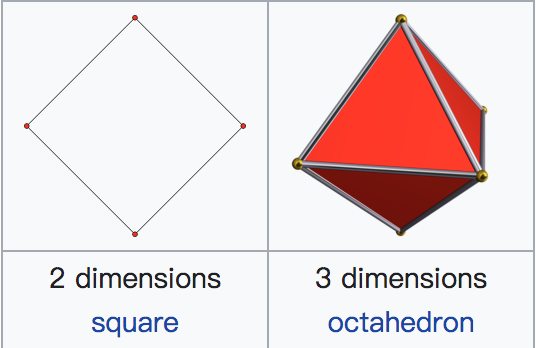
\includegraphics[width=7cm,height = 3cm]{2-3.png}
  \caption{cross-polytope examples in 2,3 dimensions}
\end{figure}

\begin{figure}[!htb]
\centering
  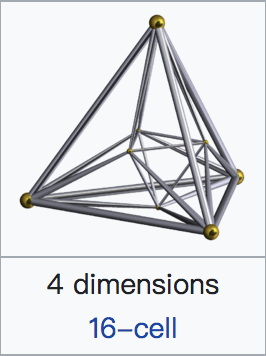
\includegraphics[width=3cm,height = 3cm]{4.png}
  \caption{cross-polytope examples in 4 dimensions}
\end{figure}


Example:\\
In 1 dimension the cross-polytope is simply the line segment [−1, +1], in 2 dimensions it is a square (or diamond) with vertices {(±1, 0), (0, ±1)}. In 3 dimensions it is an octahedron—one of the five convex regular polyhedra known as the Platonic solids. This can be generalised to higher dimensions with an n-orthoplex being constructed as a bipyramid with an (n-1)-orthoplex base.\\



\textbf{Unit Decomposition}: Decomposition of vectors into unit component.\\

Examples:\\
\textbf{3d}: Let i = {1, 0, 0}, j = {0, 1, 0}, and k = {0, 0, 1} be three unit vectors in the positive directions of the corresponding coordinate axes.

Then any vector  can be expressed as the linear combination of the vectors i, j and k:
\begin{align}
    \textbf{a} = \{a_x,a_y,a_z\} = a_x\{1,0,0\}+a_y\{0,1,0\}+a_x\{0,0,1\} = a_x\textbf{i}+a_y\textbf{j}+a_z\textbf{k}
\end{align}
Note that i, j and k are mutually orthogonal (perpendicular) unit vectors. The set of vectors i, j and k is called a rectangular orthogonal basis.

\begin{figure}[!htb]
\centering
  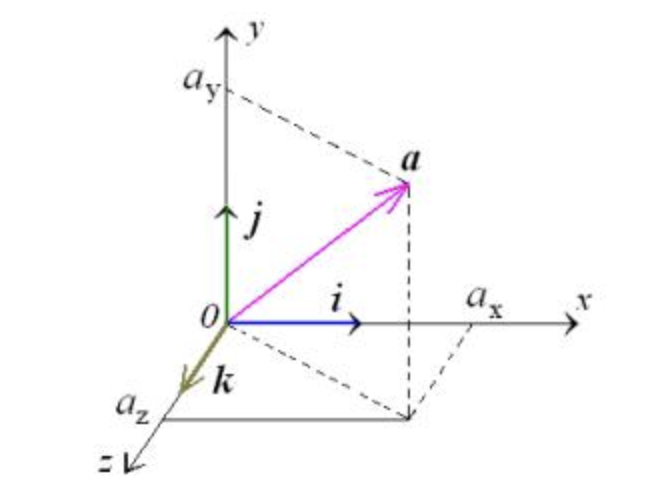
\includegraphics[width=4cm,height = 4cm]{unit-d.png}
  \caption{unit decomposition in 3 dimensions}
\end{figure}

\textbf{Gram matrix $(\Gamma)$}: In linear algebra, the Gram matrix of a set of vectors $\{v_1,...,v_n\}$ in an inner product space is the Hermitian matrix of inner products, whose entries are given by $G_{ij} = \langle v_i,v_j \rangle $\\
For finite-dimensional real vectors in $\mathbb{R}^n$ with the usual Euclidean dot product, the Gram matrix is simply $G = V^T V$,where V is a matrix whose columns are the vectors $v_k$. \\
For complex vectors in $\mathbb{C}^n$, $G = V^H V$, where $V^H$ is the conjugate transpose of V.
Given square-integrable functions $\{l_i,i = 1,...,n\}$ between interval $t_0$ to $t_f$, the Gram matrix $G = [G_{ij}]$ is:
\begin{align}
    G_{ij} = \sum_{t_0}^{t_f} l_i(\tau)\overline{l_j}(\tau) d\tau.
\end{align}

\section{Main Theorem}
\textbf{Theorem 1.1} For any $1\leq k \leq n$ we have\\
\begin{align}
    \frac{vol \varepsilon_H_k}{vol \varepsilon_k}\geq (\frac{k}{n})^{k/2}
\end{align}

and
\begin{align}
      \frac{vol \varepsilon^{H_k}}{vol \varepsilon_k}\leq (\frac{n}{k})^{k/2}
\end{align}
, where $\varepsilon_k$ is the Euclidean unit ball of dimension k.\\
Because the bounds are sharp, then there exist a subspace $H_k$ such that the two inequalities simultaneously hold as equalities.\\


In order to prove Theorem 1.1, we need to know the property of the sets of vectors:\\

\begin{align}
    \{v_1,...,v_n\} \subset \mathbb{R}^k
\end{align}
has unit decomposition in $\mathbb{R}^k$ if the operator:
\begin{align}
    \sum_{i=1}^n v_i \bigotimes v_i
\end{align}
is the identity in $\mathbb{R}^k$.\\
For any finite set $S = \{v_1,...,v_n\}$ spans $\mathbb{R}^k$, ${A_s}^{-1/2}$ maps S to a set that gives a unit decomposition, where
\begin{align}
    A_s = \sum_{i=1}^n v_i \bigotimes v_i
\end{align}

In the following Lemma, the set of all possible vectors, whose coordinates are squared lengths of the vectors give unit decomposition in $\mathbb{R}^k$ is described.\\

Remark: Kronecker product: generalization of outer product from vectors to matrix. $A\bigotimes B$ means

\begin{figure}[!htb]
\centering
  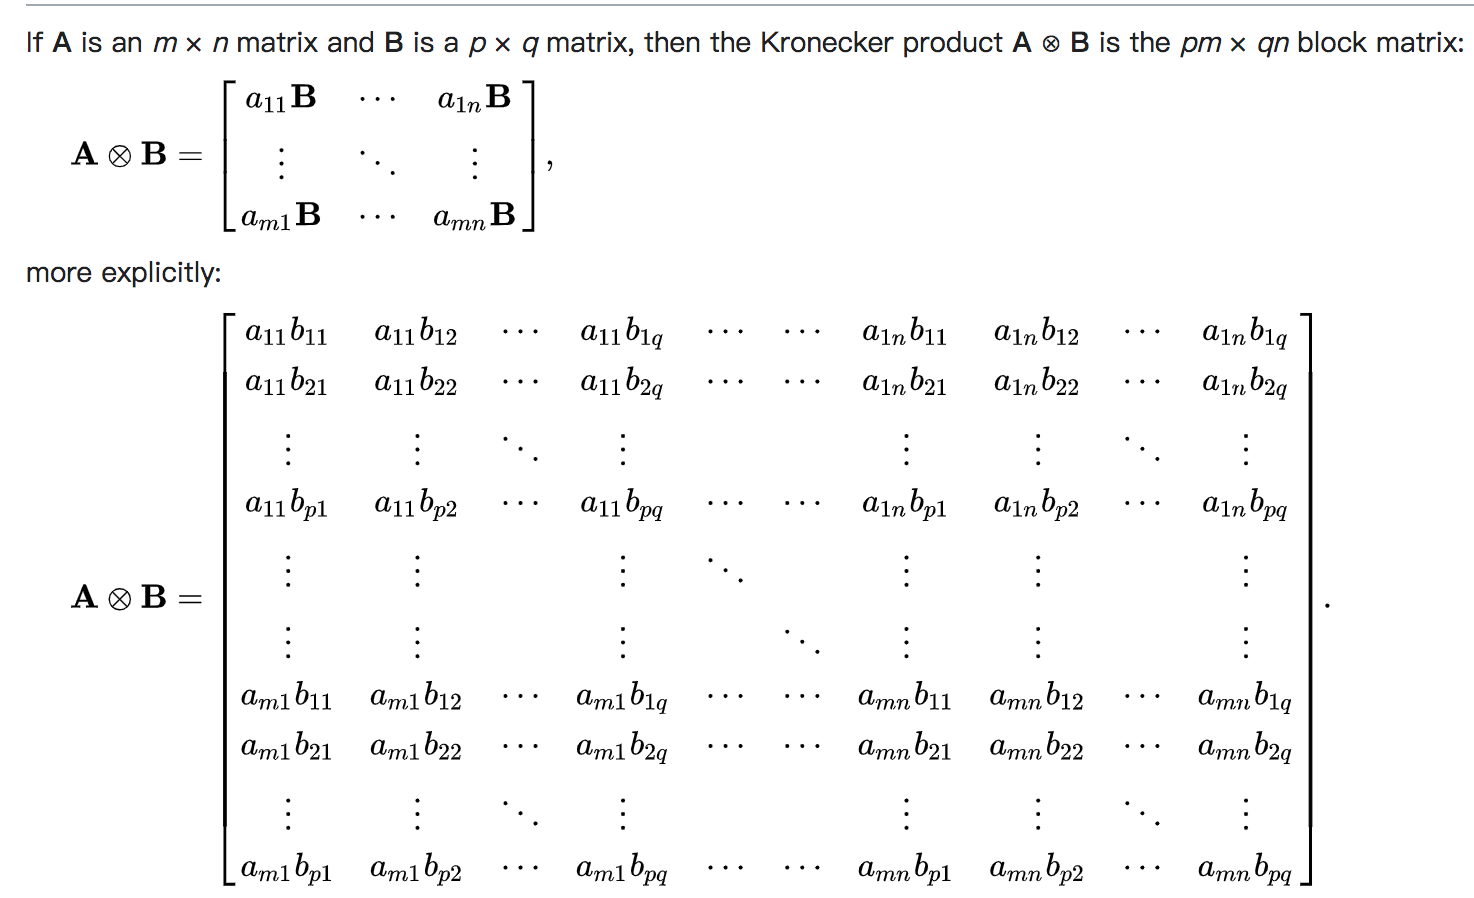
\includegraphics[width=4cm,height = 4cm]{Kronecker_product.png}
  \caption{how to compute $A\bigotimes B$}
\end{figure}

\subsection{Properties of a Unit Decomposition}\\
The following trivial lemma describes equibalent conditions for a set of vectors to give a unit decomposition.\\

\textbf{Lemma 2.1} The following assertions are equivalent:\\
(1) vectors $(v_i)^n_1$ give a unit decomposition in $\mathbb{R}^k$ ;\\
(2) there exists an orthonornal basis{$f1,...,fn$} in $\mathbb{R}^k$ such that $v_i$ is the orthogonal projection of $f_i$ onto $\mathbb{R}^k$, for any $i \in [n]$;\\
(3) Lin ${v_1,...,v_n} = \mathbb{R}^k$ and the Gram matrix $\gamma$ of ${v-1,...,v_n} \subset \mathbb{R}^k$ is the matrix of a projection operator from $\mathbb{R}^n$ onto the linear hull of the rows of the matrix $M = (v_1,...,v_n)$;\\
(4) the $k \times n$ matrix $M = (v_1,...,v_n)$ is a sub-matrix of an $n \times n$ orthogonal matrix.\\

Here we know $\mathbb{R}^k \subset \mathbb{R}^n$ as the subspace of vectors, whose last $n-k$ coordinates are zero, and $(v_i)^n_1 \subset \mathbb{R}^k \subset \mathbb{R}^n $\\

\subsection{Realizable}
\textbf{Definition 2.2} We will say that a vector $C=(c_1,...,c_n)$ is realizable in $\mathbb{R}^k$ if there exist vector $(v_i)^n_1$ which give a unit decomposition in $\mathbb{R}^k$ such that $c_i = |v_i|^2$, $i \in [n]$.

\subsection{majorize}
\textbf{Definition 2.3} Let a and b be non-negative vectors in $\mathbb{R}^n$. The vecotr a majorizes the vector b, which we denote by $a \prec b$, if the sum of the t largest entries of a is at least the sum of the t largest entries of b, for every t $\in$ n, and the sums of all entries of a and b are equal.\\
Example: \\
\begin{align*}
     a = (1,8,9)\\
    b = (5,9,4)\\
    t = 1: 9 = 9\\
    t = 2: 9+8 > 9+5\\
    sum (t=3): 1+9+8 = 5+9+4
    b \prec a
\end{align*}


\textbf{Lemma 2.4} A vecotr $(c_1,...,c_n)$ is realizable, iff
\begin{align}
    (\underbrace{1,...,1}_{k},\underbrace{0,...,0}_{n-k}) \prec (c_1,...,c_n)
\end{align}

If we prove this Lemma is true, then the vector $(\frac{k}{n},...,\frac{k}{n})$ is realizable.\\

\textbf{Proof:}\\
First let $(c_1,...,c_n)$ be realizable.\\
By definition and Lemma 2.1, there are vectors $(v_i)^n_1 \subset \mathbb{R}^k$ that gives a unit decomposition in $\mathbb{R}^k$ such that diagonal entries of Gram matrix are $(c_i)^n_1$, where the gram matrix of a projection operator from $
\mathbb{R}^k$ onto some k-dimensional subspace $H_k$.\\
So vector $(c_1,...,c_n)$ is realizable iff there exists a projection operator from $mathbb{R}^n$ onto some k-dimensional subspace with $(c_1,...,c_n)$ on the main diagonal.\\
Now applying Horn's Theorem:\\
assert $(c_1,...,c_n)$ to the main diagonal of Hermitian natrix with a vector of eigenvalues $(c\lambda_1,...,\lambda_n)$ iff $\lambda \prec c$, to the vector $(\underbrace{1,...,1}_{k},\underbrace{0,...,0}_{n-k})$.\\
Thus the proof is complete.$\msquare{}$\\


If $(v_i)^n_1 \subset \mathbb{R}^k$ are non-zero vectors, then it's unit decomposition in $\mathbb{R}^k$ iff unit vector $u_i = \frac{v_i}{\norm{v_i}}$ and positive number $c_i = |v_i|^2$ satisfied the John's condition:\\
\begin{align}
     \sum_{i=1}^n c_i u_i \bigotimes u_i = Id
\end{align}
Remark: Recall that Id represents \textbf{Identity Map}, which means $Id(x) = x$.\\


Thus in Lemma 2.4 the set of all possible vectors $(c_1,...,c_n)$ is described.



\section{Estimation for the Volume of the John-Löwner Ellipsoid}

\textbf{Lemma 3.1} Suppose that vector $(v_i)^n_1 \subset \mathbb{R}^k$ give a unit decomposition in $\mathbb{R}^k$.\\
Then for any ellipsoid $\varepsilon$ centered at the origin that covers all vectors $(v_i)^n_1$ we have:\\
\begin{align}
    vol \varepsilon \geq (\frac{k}{n})^{k/2}vol \varepsilon_k
\end{align}
where $\varepsilon_k$ is the unit ball in $\mathbb{R}^k$. The bound is tight. The inequality becomes equality iff $|v_i|^2 = \frac{k}{n}$ for all $ i\in [n]$.\\

proof:\\
Since the volume of the ellipsoid $\{x \in \mathbb{R}^k|\langle Ax,x \rangle \leq 1\}$ is $\frac{vol\varepsilon_k}{\sqrt{det A}}$ for any positive definite A on $\mathbb{R}^k$, it is enough to show that $\langleAv_i,v_i\rangle \leq 1$ for $i \in [n]$, $det A \leq (\frac{n}{k})^k$ for any positive definite A.\\
We first choose a new orthonormal basis:\\

\begin{align}
   A = diag\{\lambda_1,...,\lambda_k\}
\end{align}
in this basis in $\mathbb{R}^k$.\\
Let $v_i'$be the coordinate vector of $v_i$ for $i \in [n]$. Now in the new basis $\langleAv_i,v_i\rangle \leq 1$ has the form:\\

\begin{align}
    \sum_{j=1}^n \lambda_jv_i'[j]^2 \leq 1
\end{align}

where $v_i'[j]^2$ is the jth coordinate of $v_i'$.\\

By Lemma 2.1(4), $\sum_{j=1}^n v_i'[j]^2$ = 1. Thus we have $\sum_{j=1}^n \lambda_j \leq n$. 
By inequality of arithmetic and geometric means:\\
\begin{align}
    det A = \prod_{1}^k \lambda_i \leq (\frac{\sum_{i = 1}^k \lambda_i}{k})^k \leq (\frac{n}{k})^k
\end{align}
Then by Lemma 2.4, $(\frac{k}{n},...,\frac{k}{n})$ is realizable. Inequality (10)becomes equality. And also because of the properties of inequality of arithmetic and geometric means, the equality holds iff $\lambda_i = \frac{n}{k}$ for all i $\in$ [n].\\
By (12), the equality for (10) holds iff $|v_i|^2 = \frac{k}{n}$ for all i $\in$ [n].\\
Thus we complete the proof.
\vskip 1cm
\textbf{Now within above lemmas and theorems, we can prove Theorem 1.1 is true.}\\

\subsection{Proof of Theorem 1.1}
First fix the k-dimensional subspace $H_k$ in $\mathbb{R}^n$.\\
Let P: $\mathbb{R}^n \longrightarrow H_k$ be the projection onto $H_k$
The projection of $\diamond{}^n$ onto $H_k$: absolute convex hull of the vectors:
\begin{align}
    v_i = P e_i
\end{align}
for $i \in [n]$, $(e_i)^n_1$ is the standard basis in $\mathbb{R}^n$.\\
By Lemma 2.1, $(v_i)^n_1$ gives a unit decomposition in $\mathbb{R}^k$, and thus the volume of $\varepsilon_H_k$ is at least $(\frac{k}{n})^{k/2}vol\varepsilon_k$ by Lemma 3.1.\\
By simple duality arguments, let K be a convex body in $\mathbb{R}^n$, and define its polar body:

\begin{align}
   K^\circ = \{y|xy\leq 1 \forall x \in K\}
\end{align}
for a given k-dimension subspace $H_k$ with the origin in its interior, we have:\\
the polar of $(K\cap H_k)$ as the subset of $H_k$ is the projection of $K^\circ$ onto $H_k$; and the polar ellipsoid of the John ellipsoid of K is the Löwner ellipsoid of $K^\circ$, the product of the volums of them is $vol^2\varepsilon_k$.\\
Because $\msquare{}^n$ is the polar of $\diamond{}^n$, the upper bound of the volume of the John ellipsoid of k-dimensional section of $\msquare{}^n$.
Thus we complete the proof.

\section{Bounds of the Volume}

In Ball's fundamental paper we have proved the following:\\
\begin{align}
    \frac{vol(\msquare{}^n \cap H_k)}{vol\msquare{}^k} \leq (\frac{n}{k})^{k/2}
\end{align}
and
\begin{align}
    \frac{vol(\msquare{}^n \cap H_k)}{vol\msquare{}^k} \leq \frac{vol \varepsilon^{H_k}}{vol\varepsilon_k}
\end{align}
for any $H_k \subset \mathbb{R}^n$. The dual ineaulities proved by Barthe is:
\begin{align}
    \frac{vol(\diamond{}^n| H_k)}{vol\diamond{}^k} \geq (\frac{n}{k})^{k/2}
\end{align}
and
\begin{align}
    \frac{vol(\diamond{}^n | H_k)}{vol\diamond{}^k} \geq \frac{vol \varepsilon^{H_k}}{vol\varepsilon_k}
\end{align}
which is also called left-hand side inequalities.\\

Noted that left-hand side inequalities are optimal when k divides n so that there exists such $H_k$ make the equalities hold. This is followed from right-hand side inequalities and Theorem 1.1.\\
If the left-hand side inequalities are tight, then we have right hand side inequalities are tight as well for $H_k$, and the ellipsoids have the maximum possible volume. Thus we can settle all the equality cases in the left-hand side inequalities.
Inequalities (16),(17),(18),(19) becomes eqaulities iff k diveds n, $H_k$ is determined by coordinate permutation and change of sign:
\begin{align}
    x_{\frac{n}{k}j+i_1} =  x_{\frac{n}{k}j+i_2}
\end{align}
where $j \in \overline{0,k-1}$ and $1\leq i_1$,$i_2 \leq \frac{n}{k}$.

\section{References}
1.Grigory Ivanov: On the Volume of the John-Löwner Ellipsoid,pp 455-459,Springer Science+Business Media, LLC, part of Springer Nature 2019\\
2.Martin Henk:Lowner–John Ellipsoids,2010 Mathematics Subject Classification: 52XX, 90CXX,pp.95-103\\
3. Ball,K.:Volumes of sections of cubes and related problems. In:Lindenstrauss,J.,Milman,V.D.(eds.)Geometric Aspects of Functional Analysis.Lecture Notes in Mathematics, pp.251-260. Springer, Berlin(1989)\\
4.en.wikipedia.org/wiki/Cross-polytope

\end{document}
